\documentclass{article}
\usepackage[margin=0.25in]{geometry}
\usepackage{graphicx}% http://ctan.org/pkg/graphicx
\usepackage{array}% http://ctan.org/pkg/array
\usepackage[utf8]{inputenc}
\usepackage[T2A]{fontenc}

\begin{document}
\centering
\textbf{Тренировка А - крака, корем}\\
%Групи: 1+2; 3+4+5;6+7;\\ 
\begin{tabular}{ | m{5cm} | m{5cm} | m{5cm} | }
\hline
1. Клек с щанга & 2. Напади с дъмбели & 3. Планк \\ 
\begin{minipage}{5cm} 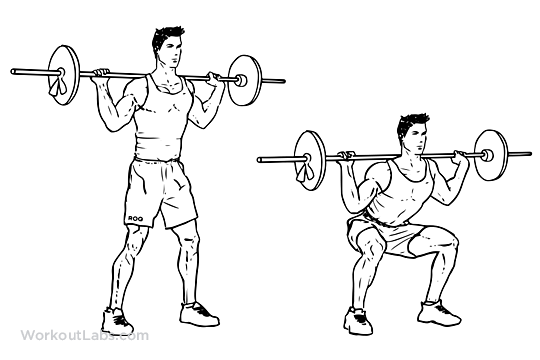
\includegraphics[width=\linewidth, height=60mm]{Barbell-Squat.png}\end{minipage}&
\begin{minipage}{5cm} 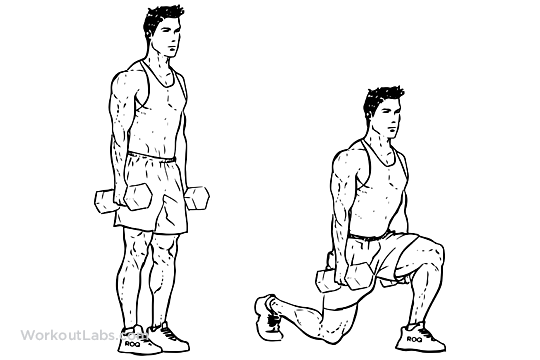
\includegraphics[width=\linewidth, height=60mm]{Dumbbell_Lunges.png} \end{minipage}& 
\begin{minipage}{5cm} 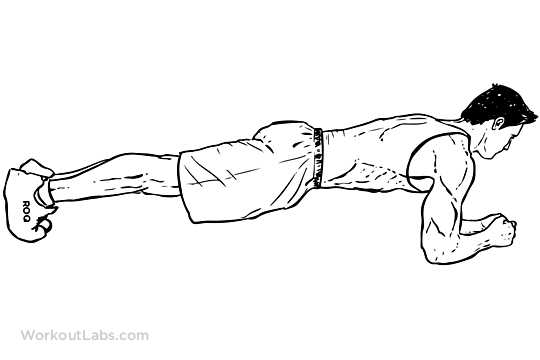
\includegraphics[width=\linewidth, height=60mm]{front-plank.png} \end{minipage}\\ 
3 х 20-30 reps & 2 х 15-20 на крак; & 3 x 45 сек - 2 мин \\
\hline
4. Глутеус мост на един крак & 5. Мъртва тяга с пудовка & 6. Абдуктор \\ 
\begin{minipage}{5cm} 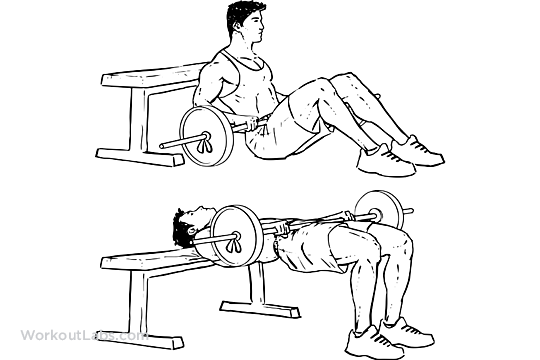
\includegraphics[width=\linewidth, height=60mm]{Barbell_Hip_Thrusts.png} \end{minipage} & 
\begin{minipage}{5cm} 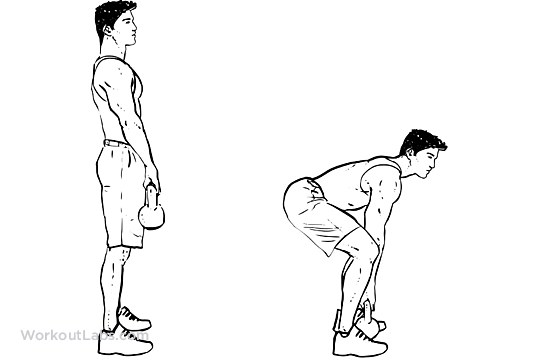
\includegraphics[width=\linewidth, height=60mm]{Kettlebell_Deadlifts.png} \end{minipage} &
\begin{minipage}{5cm} 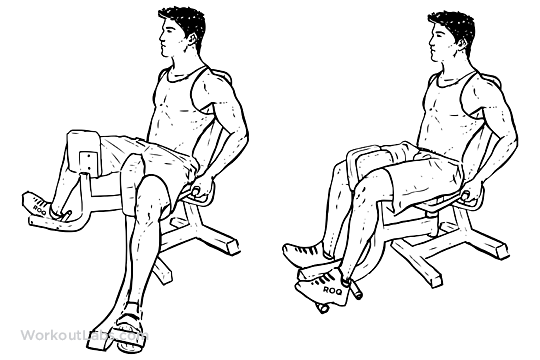
\includegraphics[width=\linewidth, height=60mm]{Adductor.png} \end{minipage} \\
3 х 15-25 на крак &  3 х 20-30 reps & 2 х 50 Отваряне + 3 x 33 Затваряне  \\ 
\hline
\end{tabular}
\begin{tabular}{ | m{4cm} | m{4cm} | m{4cm} |  m{4cm} | }
\hline
Повдигане на краката от стенд с дъмбел&  Коремна на колене & Руско & Ротация с кабел \\ 
\begin{minipage}{4cm} 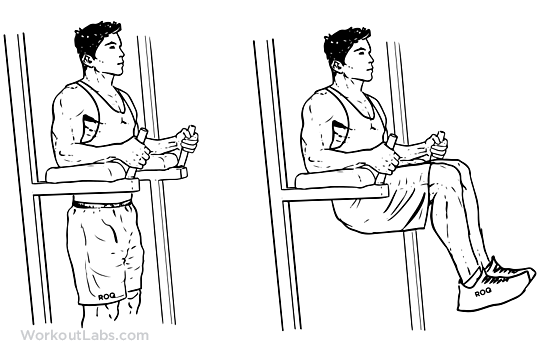
\includegraphics[width=\linewidth, height=50mm]{Knee_Hip_Raise.png} \end{minipage} & 
\begin{minipage}{4cm} 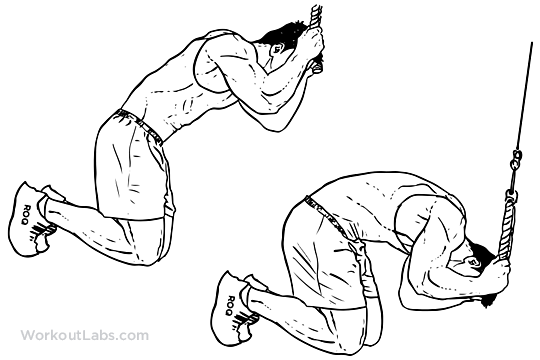
\includegraphics[width=\linewidth, height=50mm]{Kneeling_Cable_Crunch.png} \end{minipage} &
\begin{minipage}{4cm} 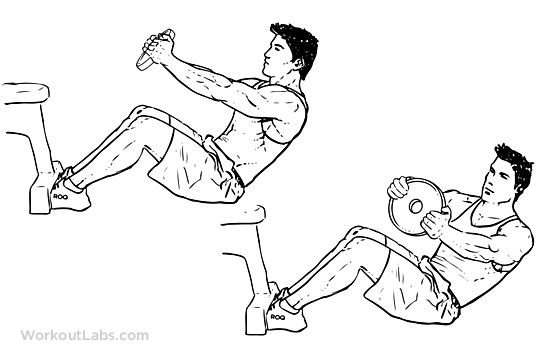
\includegraphics[width=\linewidth, height=50mm]{Russian_Twist.png} \end{minipage} & 
\begin{minipage}{4cm} 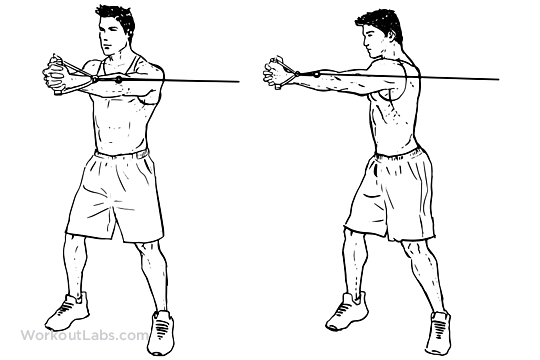
\includegraphics[width=\linewidth, height=50mm]{Cable_Core_Rotation.png} \end{minipage} \\
3-4 х 6-15 reps & 3-4 x 6-15 reps & 3-4 х 6-15 reps & 3-4 x 6-15 reps \\ 
\hline
\end{tabular}
\newpage
\textbf{Ден В: Гръдно-раменна, корем}\\
%Загрявка 5 мин. кардио + 2 мин. развъртане на стави (лакти, китки, рамене ,
%раменен пояс, таз, колене, глезени, кръст)\\
%Загряващи серии 1 х 12-15 за всяко първо движение за мускулна група с малка
%тежест\\
%Групи: 1+2; 3+4+5; 6+7; 8; 9\\ 
\begin{tabular}{ | m{5cm} | m{5cm} | m{5cm} | }
\hline
1. Избутване на тренажор за гръдна мускулатура & 
2. Избутване на машина за гърди & 
3. Затваряне на пек-дек машина\\ 
\begin{minipage}{5cm} 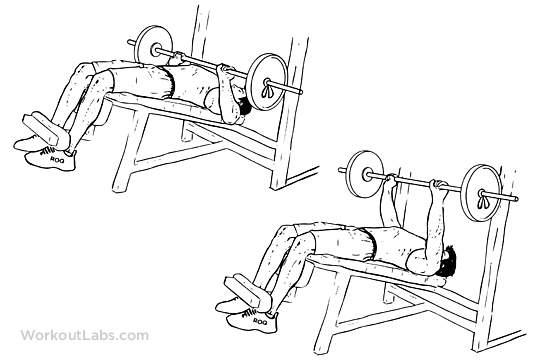
\includegraphics[width=\linewidth, height=60mm]{Decline_Barbell_Bench_Press.png} \end{minipage}&
\begin{minipage}{5cm} 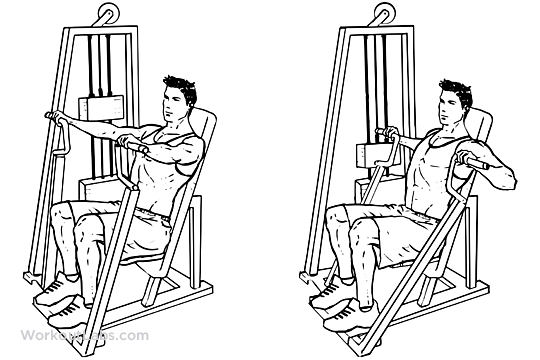
\includegraphics[width=\linewidth, height=60mm]{Hammer_Strength_Machine_Chest.png} \end{minipage}& 
\begin{minipage}{5cm} 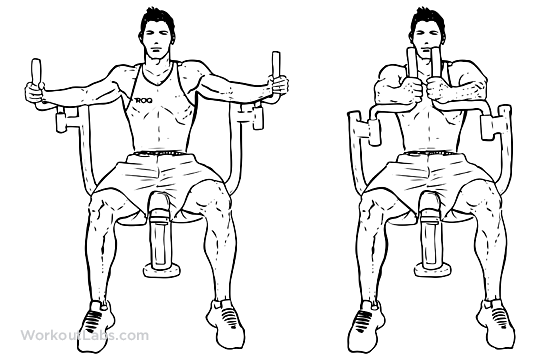
\includegraphics[width=\linewidth, height=60mm]{Butterfly.png} \end{minipage}\\ 
1 х 20 загряваща + 4 х 7-10 &  4 х 8-10 reps & 4 х 12-15 reps \\
\hline
\end{tabular}

\begin{tabular}{ | m{4cm} | m{4cm} | m{4cm} |  m{4cm} | }
\hline
4. Раменни преси на смит машина (лакти под китки) & 
5. Разтваряне на ръцете на пек-бек машина & 
6. Повдигане на ръцете напред от седеж & 
7. Повдигане на ръцете встрани от седеж \\ 
\begin{minipage}{4cm} 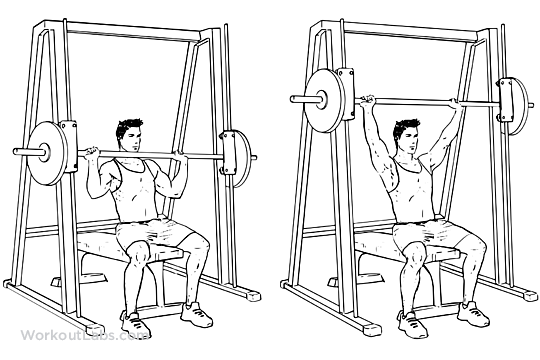
\includegraphics[width=\linewidth, height=50mm]{Smith_Machine_Shoulder_Press.png} \end{minipage} & 
\begin{minipage}{4cm} 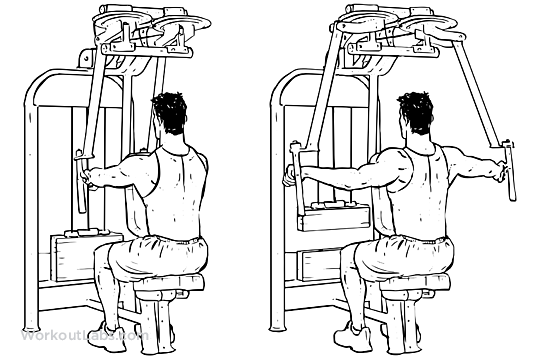
\includegraphics[width=\linewidth, height=50mm]{Rear_Delt_Flyes_Machine.png} \end{minipage} &
\begin{minipage}{4cm} 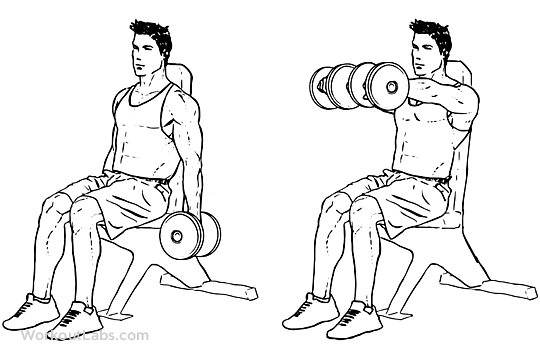
\includegraphics[width=\linewidth, height=50mm]{Seated_Dual_Front_Raises.png} \end{minipage} & 
\begin{minipage}{4cm} 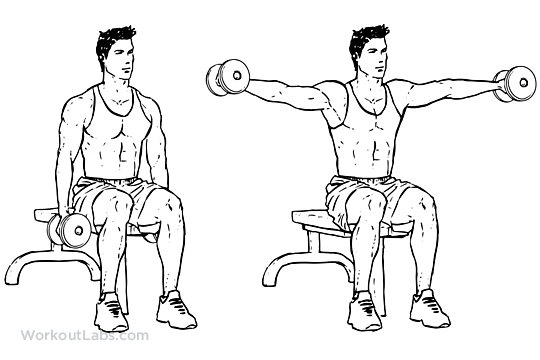
\includegraphics[width=\linewidth, height=50mm]{Seated_Lateral_Dumbbell_Raise.png} \end{minipage} \\
4 х 8-12 reps & 3 x 10-12 reps & 2 х 8-12 reps & 2 x 8-12 reps \\ 
\hline
Повдигане на краката от стенд с дъмбел&  Коремна на колене & Руско & Ротация с кабел \\ 
\begin{minipage}{4cm} 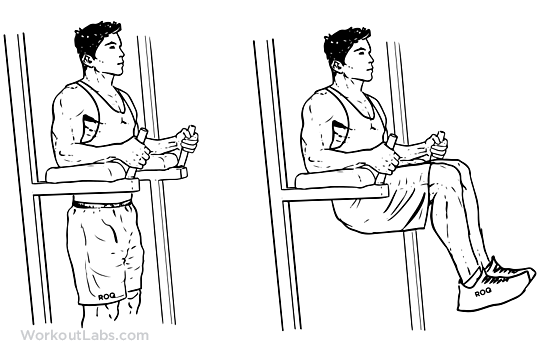
\includegraphics[width=\linewidth, height=50mm]{Knee_Hip_Raise.png} \end{minipage} & 
\begin{minipage}{4cm} 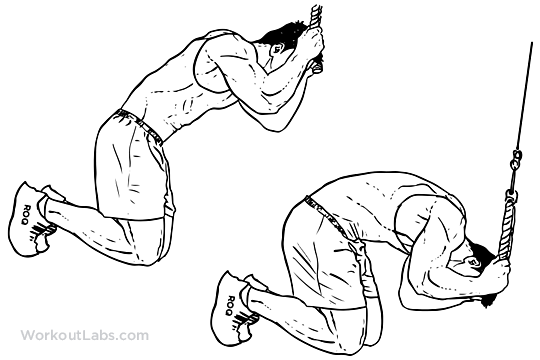
\includegraphics[width=\linewidth, height=50mm]{Kneeling_Cable_Crunch.png} \end{minipage} &
\begin{minipage}{4cm} 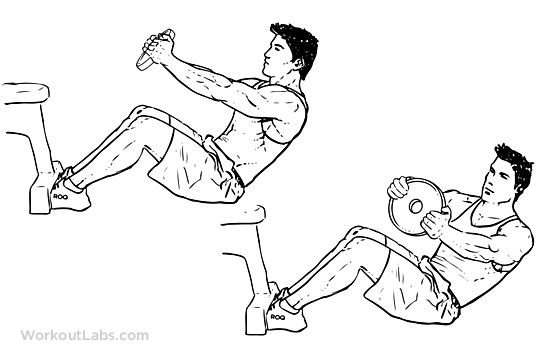
\includegraphics[width=\linewidth, height=50mm]{Russian_Twist.png} \end{minipage} & 
\begin{minipage}{4cm} 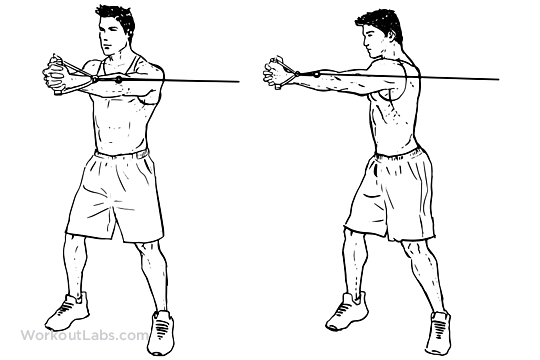
\includegraphics[width=\linewidth, height=50mm]{Cable_Core_Rotation.png} \end{minipage} \\
3-4 х 6-15 reps & 3-4 x 6-15 reps & 3-4 х 6-15 reps & 3-4 x 6-15 reps \\ 
\hline
\end{tabular}

%\newpage
%\textbf{Ден С: седалищна, бедрена мускулатура и коремен пояс}\\
%Загрявка 5 мин. кардио + 2 мин. развъртане на стави (лакти, китки, рамене ,
%раменен пояс, таз, колене, глезени, кръст)\\
%Загряващи серии 1 х 12-15 за всяко първо движение за мускулна група с малка
%тежест\\
%Групи: 1+2; 3+4+5;6+7;\\ 
%\begin{tabular}{ | m{5cm} | m{5cm} | m{5cm} | }
%\hline
%1. Полуклек до пейка със собствено тегло & 
%2. Преден планк   & 
%3  Добро утро с прави крака и диск/дъмбели\\ 
%\begin{minipage}{5cm} 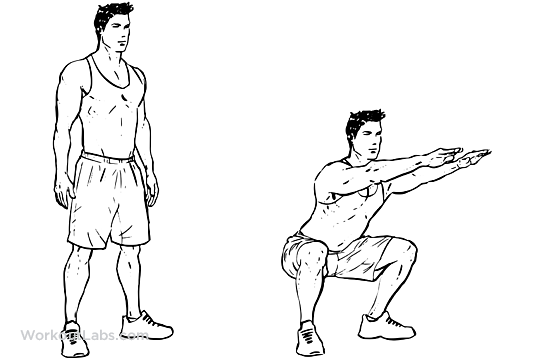
\includegraphics[width=\linewidth, height=60mm]{day_C_ex_1_Air_Squats.png} \end{minipage}&
%\begin{minipage}{5cm} 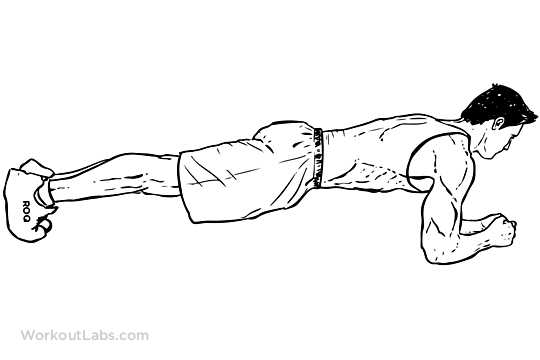
\includegraphics[width=\linewidth, height=60mm]{day_C_ex_2_front-plank.png} \end{minipage}& 
%\begin{minipage}{5cm} 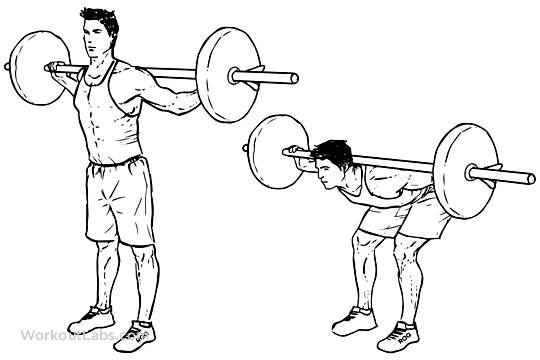
\includegraphics[width=\linewidth, height=60mm]{day_C_ex_3_Barbell_Good_Morning.png} \end{minipage}\\ 
%3-4 х 15-30 reps &  2-3 х 40-90 сек &  2-3 х 12-20 reps \\
%\hline
%4. Страничен планк  & 
%5. Катерач (облегнати на пейка) & 
%6. Абдуктор машина \\ 
%\begin{minipage}{5cm} 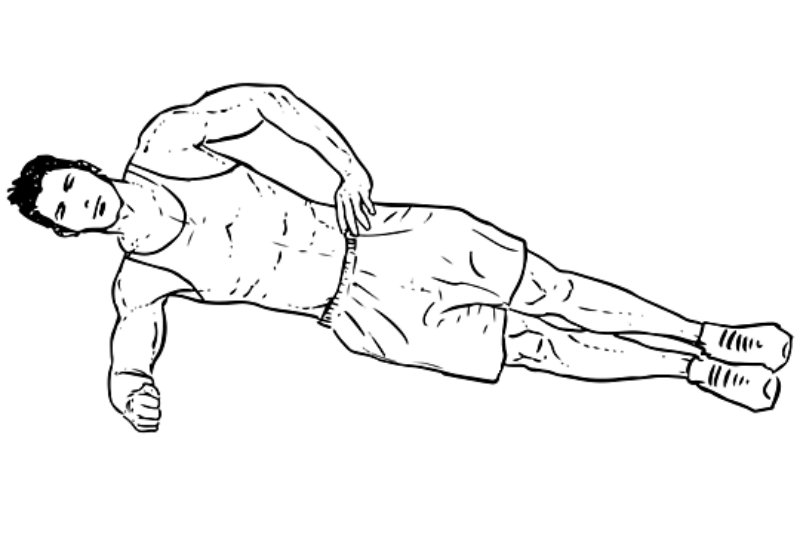
\includegraphics[width=\linewidth, height=60mm]{day_C_ex_4_Side-Plank.png} \end{minipage} &
%\begin{minipage}{5cm} 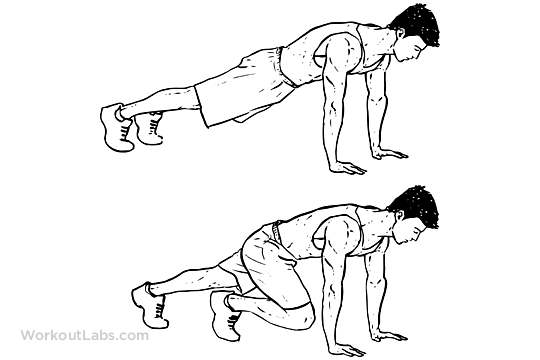
\includegraphics[width=\linewidth, height=60mm]{day_C_ex_5_Mountain_Climbers.png} \end{minipage} & 
%\begin{minipage}{5cm} 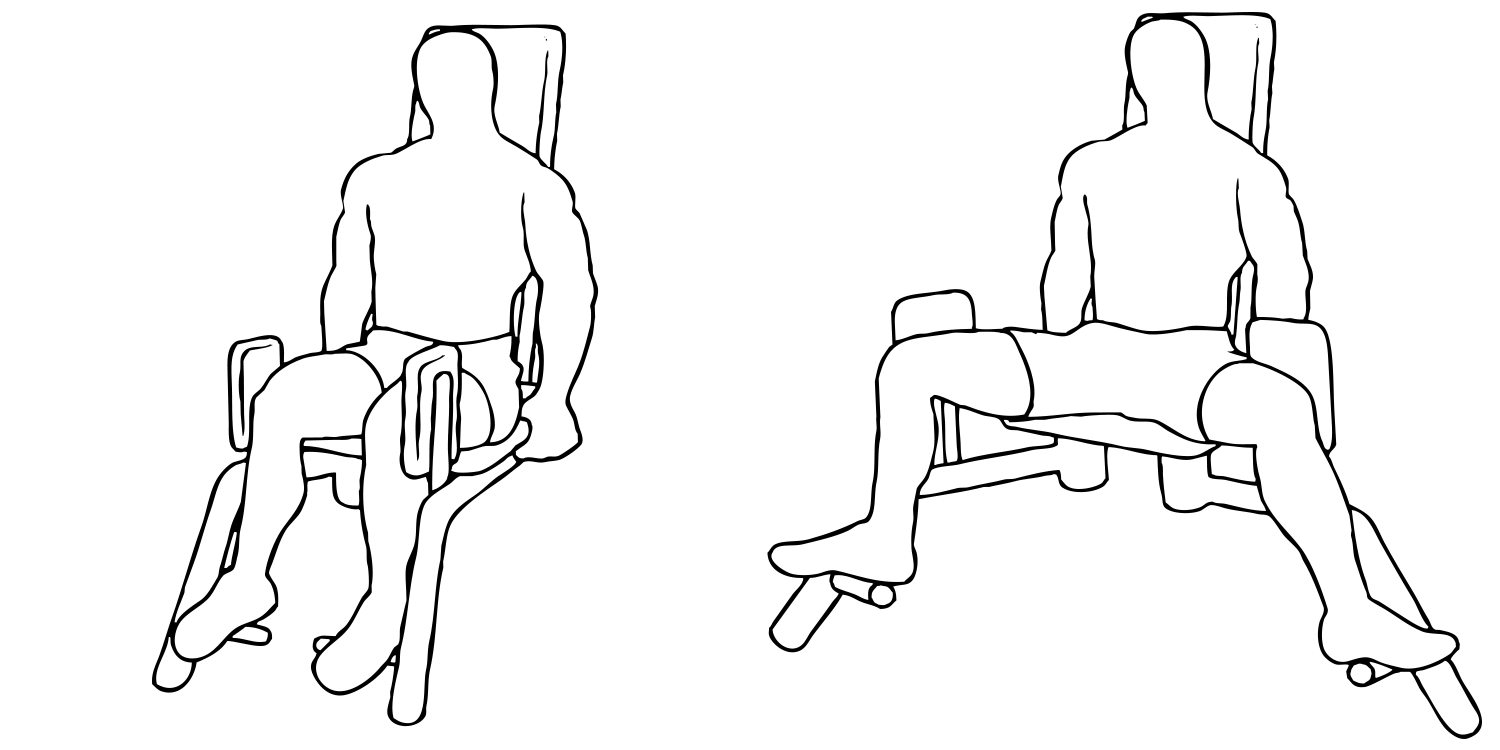
\includegraphics[width=\linewidth, height=60mm]{day_C_ex_6_winner-thigh-abductor.png} \end{minipage} \\
%2-3 х 30-60 сек вляво и вдясно & 2-3 х 30 странично + 30 фронтално & 2 х 30-50 Отваряне + 30-50 Затваряне \\ 
%\hline
%7. Руско извиване (наклона варира според теглото на атлета)& 
%8. Задна опора & 
%9. Кардио\\ 
%\begin{minipage}{5cm} 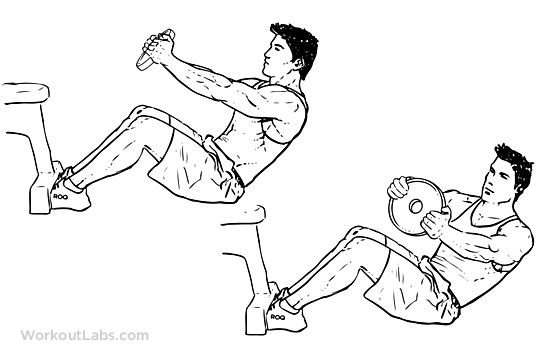
\includegraphics[width=\linewidth, height=60mm]{day_C_ex_7_Russian_Twist.png} \end{minipage} &
%\begin{minipage}{5cm} 
\includegraphics[width=\linewidth, height=60mm]{day_C_ex_8_reverse-plank.jpg} \end{minipage} & 
%\begin{minipage}{5cm} 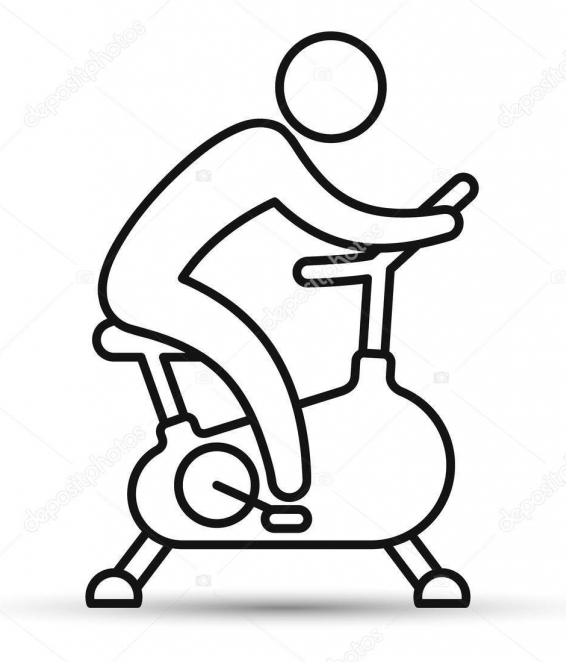
\includegraphics[width=\linewidth, height=60mm]{day_C_ex_9_cardio.jpg} \end{minipage} \\
%2 х 20-30 с 2-3 сек. въртене в посока;& 2 х 30-60 сек & ~20 (до 40) минути \\ 
%\hline
%\end{tabular}

\end{document}
